\documentclass{beamer}
\usepackage[utf8]{inputenc}
\usepackage[T1]{fontenc}
\usepackage{ragged2e}

\usepackage[utf8]{inputenc}  
\usepackage[T1]{fontenc}
\usepackage{geometry}
\usepackage{listings}
\usepackage{url}
\usepackage{hhline}
\usepackage[normalem]{ulem}
\usepackage[font={color=foreground,bf}]{caption}
\usepackage{array,booktabs,arydshln}
\usepackage{pdflscape}
\usepackage{xcolor}
\usepackage{inconsolata}
\usepackage{pgfplots}
\usepackage{listings}
\pgfplotsset{compat=1.17}
\usetikzlibrary{shadows}

\def\imgBaseDir{img}
\def\imgSubDir{}
\newcommand\setimgdir[1]{\def\imgSubDir{#1/}}

\newcommand\img[1]{\includegraphics[width=\linewidth]{\imgBaseDir/\imgSubDir#1}}

\newcommand\darktheme {
	
	\colorlet{foreground}{black!25}
	\colorlet{background}{black!74}
	\colorlet{focus}{yellow!50}
	\definecolor{codeColor}{RGB}{85,255,85}
	\colorlet{codeBackground}{black!80}
	\def \imgBaseDir {imgDark}
	
	
	
}
%\rowcolors{1}{background}{background!95} % Alternated array colors
%%%%%%%%%%%%%%%%%%%%%%%%%%%%%%%%%%%%%%%%%%%%%%%%%%%%%%%   BASIC STYLES   %%%%%%%%%%%%%%%%%%%%%%%%%%%%%%%%%%%%%%%%%%%%%%%%%%%%%%%
\colorlet{foreground}{black}
\colorlet{background}{white}
\colorlet{focus}{blue}
%\definecolor{codeColor}{RGB}{0,0,0}
\colorlet{codeBackground}{black!10}



\renewcommand\emph[1]	{{ \color{red!40}	\textbf{#1}} 			}
\newcommand\mynote[1]	{{ \color{focus!50} \textbf{NOTE:	} #1 }\\}
\newcommand\warning[1]	{{ \color{focus!70} \textbf{WARNING:} #1 }\\}
\newcommand\todo[1]		{{ \color{focus} 	\textbf{TODO:} 	  #1 }\\}
%%%%%%%%%%%%%%%%%%%%%%%%%%%%%%%%%%%%%%%%%%%%%%%%%%%%%%%   CODE   %%%%%%%%%%%%%%%%%%%%%%%%%%%%%%%%%%%%%%%%%%%%%%%%%%%%%%%
\lstset{
	firstnumber=1,
	texcl=true,inputencoding=latin1,
	backgroundcolor=\color{codeBackground},   % choose the background color; you must add \usepackage{color} or \usepackage{xcolor}; should come as last argument,
	basicstyle=\footnotesize\ttfamily,      % the size of the fonts that are used for the code
	breakatwhitespace=true,         % sets if automatic breaks should only happen at whitespace
	breaklines=true,
	captionpos=b,                    % sets the caption-position to bottom
	commentstyle=\color{green!65!black},    % comment style
	deletekeywords={...},            % if you want to delete keywords from the given language
	escapeinside={\%*}{*)},          % if you want to add LaTeX within your code
	extendedchars=true,              % lets you use non-ASCII characters; for 8-bits encodings only, does not work with UTF-8
	frame=single,	                   % adds a frame around the code
	keepspaces=true,                 % keeps spaces in text, useful for keeping indentation of code (possibly needs columns=flexible)
	keywordstyle=\color{blue!60},       % keyword style
	language=C,                 % the language of the code,
	morekeywords={*,...},            % if you want to add more keywords to the set
	numbers=left,                    % where to put the line-numbers; possible values are (none, left, right)
	numbersep=5pt,                   % how far the line-numbers are from the code
	numberstyle=\tiny\color{black!40}, % the style that is used for the line-numbers
	rulecolor=\color{black},         % if not set, the frame-color may be changed on line-breaks within not-black text (e.g. comments (green here))
	showspaces=false,                % show spaces everywhere adding particular underscores; it overrides 'showstringspaces'
	showstringspaces=false,          % underline spaces within strings only
	showtabs=false,                  % show tabs within strings adding particular underscores
	stepnumber=5,                    % the step between two line-numbers. If it's 1, each line will be numbered
	stringstyle=\color{violet!50},     % string literal style
	tabsize=4,	                   % sets default tabsize to 2 spaces
	title=\lstname                   % show the filename of files included with \lstinputlisting; also try caption instead of title	
}

\newcommand\icode[1]{\lstinline[breaklines=true,breakatwhitespace=false, basicstyle=\ttfamily\small]{#1}}\lstnewenvironment{code}{}{}
\lstnewenvironment{bash}{\lstset{language=Bash}}{}
\lstnewenvironment{fcode}[1]{\lstset{caption=#1}}{}

% % Environment for list in block most common case
\newenvironment{bl}[1][] % By default, no title
	{\begin{block}{#1}\begin{itemize}}
	{\end{itemize}\end{block}}


\newcolumntype{Y}{>{\centering\arraybackslash}X}


\justifying

\newcommand{\logoWidth}{1 cm}
\newcommand{\spaceh}{0,5 cm}
\colorlet{foreground}{black}
\colorlet{background}{white}
\colorlet{focus}{blue}
%\definecolor{codeColor}{RGB}{0,0,0}
\colorlet{codeBackground}{black!10}


\title{Automatic exploit generation}
\author[shortname]{
	Maxime Bélair  \inst{1} \and
	Manh-Dung Nguyen  \inst{2} \and
	Emilien Fournier \inst{3}\and
	Tristan Benoit \inst{4}\and
	Gabriel Sauger \inst{5}\\
	\vspace{0.3cm}
	\textbf{Subject by}: \large Jules Villard - 
	
\includegraphics[width = 1cm]{Figures/Logos/FacebookLogo.png}
}

\institute{
	\inst{1}%
	Orange Labs / IMT atlantique - \tiny maxime.belair@imt-atlantique.fr
	\and
	\inst{2}%
	CEA LIST \& Université Grenoble Alpes - \tiny manh-dung.nguyen@cea.fr
	\and
	\inst{3}%
	ENSTA Bretagne / Lab-STICC - \tiny emilien.fournier@ensta-bretagne.org
	\and
	\inst{4}%
	LORIA - \tiny tristan.benoit@loria.fr
	\and
	\inst{5}%
	LORIA - \tiny gabriel.sauger@loria.fr
}
\date{}

\titlegraphic{ \vspace{-1cm}
	
	
\includegraphics[width = \logoWidth]{Figures/Logos/MaxLogo1.png}
	
\includegraphics[width = 0.5cm]{Figures/Logos/MaxLogo2.png}
	\hspace{\spaceh}
	
\includegraphics[width = 0.75cm]{Figures/Logos/MDLogo1.png}
	
\includegraphics[width = \logoWidth]{Figures/Logos/MDLogo2.png}
	\hspace{\spaceh}
	
\includegraphics[width = 2.5cm]{Figures/Logos/EmilienLogo1.png}
	\hspace{0.5cm}
	
\includegraphics[width = 2CM]{Figures/Logos/GabrielLogo1.png}
	\hspace{\spaceh}
}

\usetheme{Antibes}


\setbeamertemplate{footline}[frame number]


\begin{document}
	
	\begin{frame}
	\titlepage
\end{frame}


\section{Problem overview}

\begin{frame}
\centering
\LARGE
Problem Overview
\end{frame}

\subsection{Context}

\begin{frame}{Context}

\begin{itemize}
\item Bugs in devices
\item Are they weaknesses ?
\end{itemize}

\begin{block}{Formal challenge}
Can we automatically turn static analysis reports into executable confirming the vulnerability of a program ?
\end{block}


\end{frame}

\subsection*{Program bug example}
\begin{frame}{Program bug example}
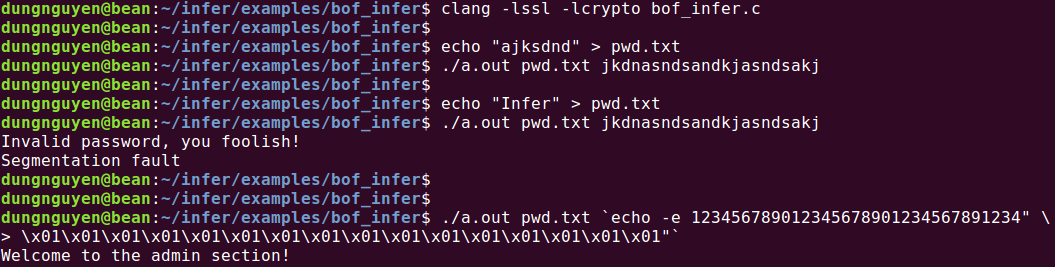
\includegraphics[width=12cm]{Figures/main.c/mainTest.png}
\end{frame}

\subsection{Infer tool}

\begin{frame}{Infer tool}

\begin{figure}

\includegraphics[width=10cm]{Figures/InferDrawing.png}
\end{figure}

\end{frame}

\begin{frame}

\begin{figure}

\includegraphics[width = 1.8cm]{Figures/InferLogo.png}

\end{figure}

\vspace{1cm}

\begin{itemize}
\item Static analysis tool from Facebook
\item \textbf{Capture} phase, then \textbf{Analysis} phase
\end{itemize}

\end{frame}

\begin{frame}{Infer tool example}

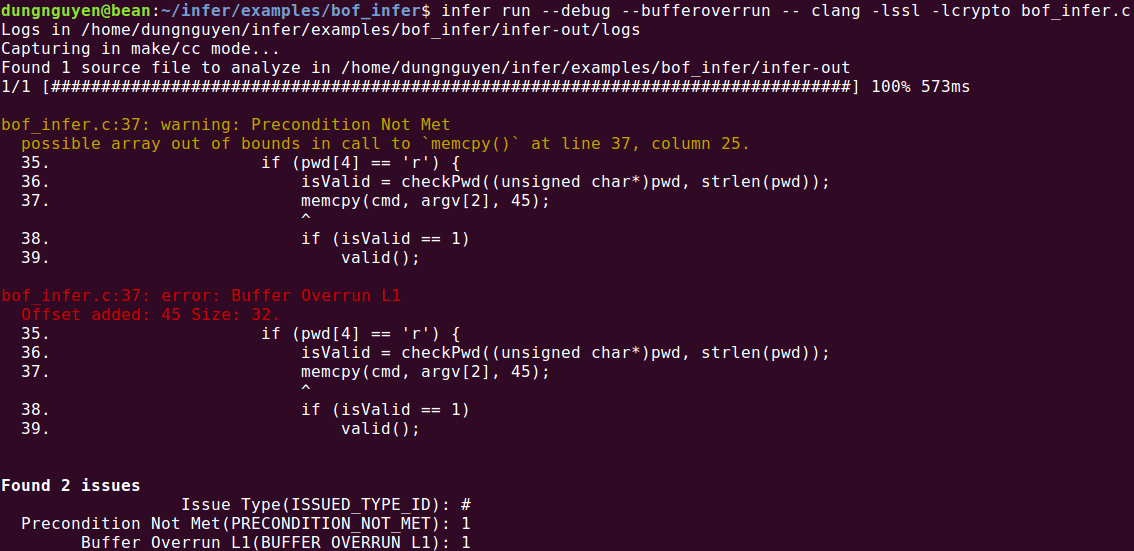
\includegraphics[width=12cm]{Figures/main.c/inferRunOnMain.png}
\end{frame}

\subsection{Practical approach}



\begin{frame}{Practical approach}

\includegraphics<1>[scale=0.3]{Figures/Workflow/1.png}
\includegraphics<2>[scale=0.3]{Figures/Workflow/2.png}
\includegraphics<3>[scale=0.3]{Figures/Workflow/3.png}
\includegraphics<4>[scale=0.3]{Figures/Workflow/4.png}

\end{frame}


\begin{frame}{Practical approach}

\begin{block}{Practical challenge}
Given the Infer information about bugs of a program A, create a program B that crashes A
\end{block}

\end{frame}

\begin{frame}{Table of content}
\tableofcontents
\end{frame}

\section{Proposed approaches}

\begin{frame}
\centering

P\LARGE roposed approaches
\end{frame}


\subsection{Model checking}

\begin{frame}{Model checking }

\begin{columns}[t]
\begin{column}{5cm}
\begin{block}{ Model Checking }
\begin{itemize}
\item Intuitive 
\item Automated 
\item Provides counter-example 
\item[$\times$] State-space explosion
\end{itemize}
\end{block}

\begin{block}{What is it ? }
\begin{itemize}
\item Fixed-point algorithm 
\item Plenty of algorithmic variations
\end{itemize}

\end{block}
\end{column}

\begin{column}{5cm}

\end{column}
\end{columns}

\end{frame}

\begin{frame}
\frametitle{}

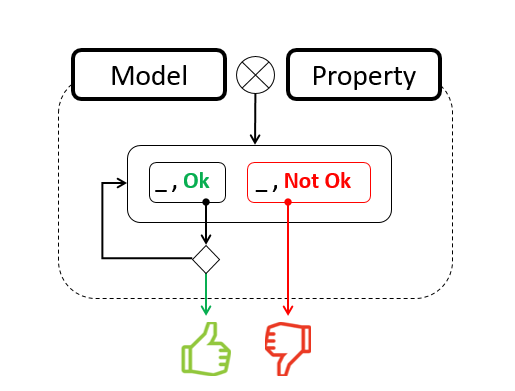
\includegraphics[width=0.8\textwidth]{Figures/Model-checking.png}



\end{frame}


\subsection{SMT solvers}

\begin{frame}{SMT solvers}

Present logic solvers

\end{frame}

\begin{frame}{SMT Solvers}
Compiler / Interpreter information
\end{frame}

\begin{frame}{SMT Solver}

\includegraphics<1>[width=9cm]{Figures/SMTsolver/1.png}
\includegraphics<2>[width=9cm]{Figures/SMTsolver/2.png}
\includegraphics<3>[width=9cm]{Figures/SMTsolver/3.png}
\includegraphics<4>[width=9cm]{Figures/SMTsolver/4.png}
\includegraphics<5>[width=9cm]{Figures/SMTsolver/5.png}
\includegraphics<6>[width=9cm]{Figures/SMTsolver/6.png}
\includegraphics<7>[width=9cm]{Figures/SMTsolver/7.png}

\end{frame}

\begin{frame}{SMT results}
Present the results we have and on which program. The performance review is NOT done here, but in Part 3/Result Comparison
\end{frame}

\subsection{Fuzzing technique}

\begin{frame}{Fuzzing technique}

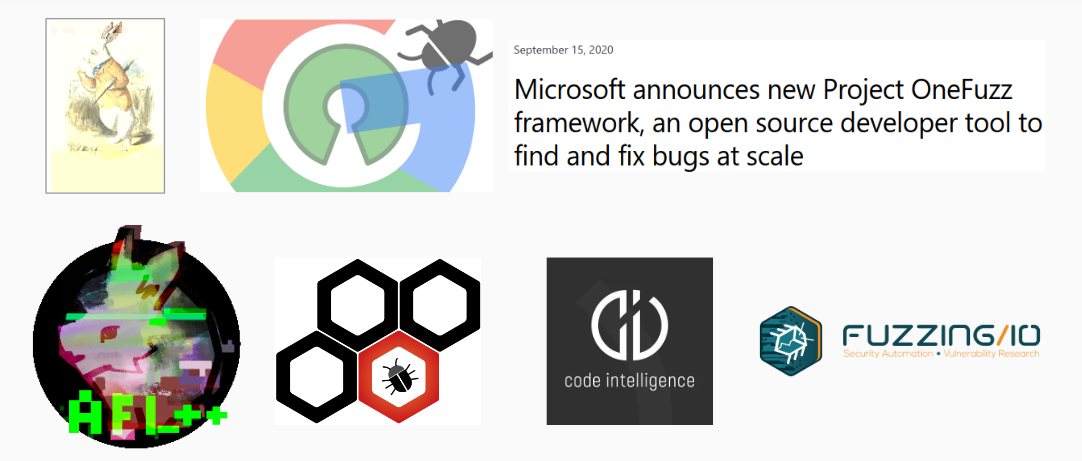
\includegraphics[width=11.5cm]{Figures/Fuzzing/graph1.png}

\end{frame}

\begin{frame}{Coverage-guided Greybox fuzzing}
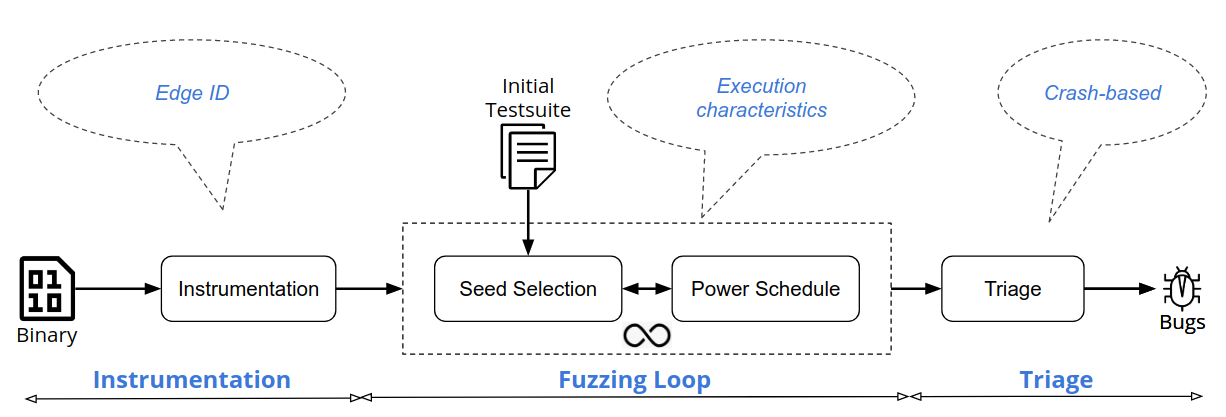
\includegraphics[width=11.5cm]{Figures/Fuzzing/graph2.png}
\end{frame}

\begin{frame}{Direct Greybox fuzzing}
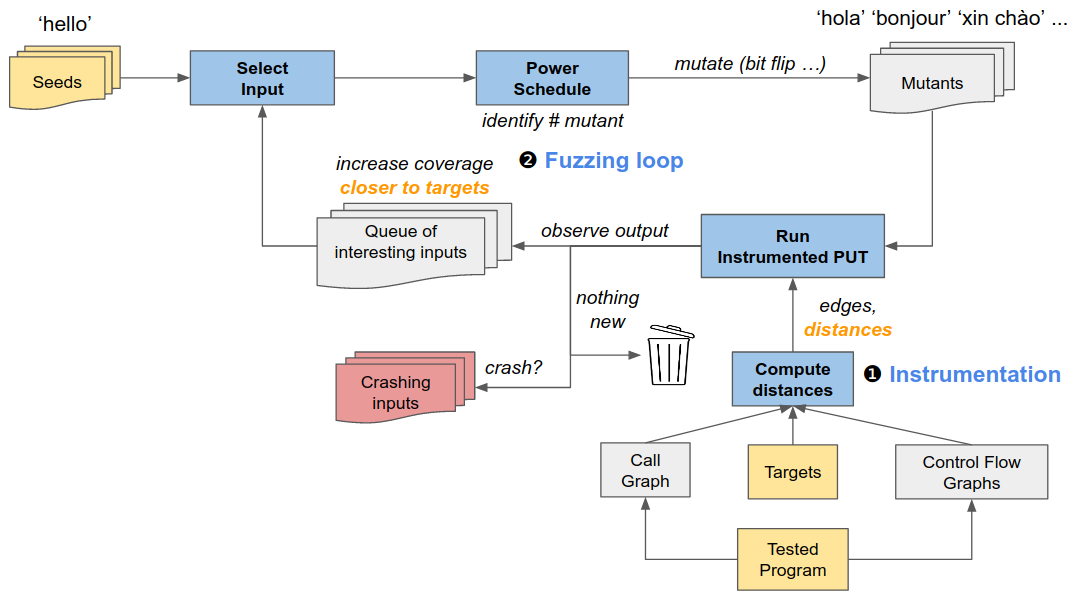
\includegraphics[width=11.5cm]{Figures/Fuzzing/graph3.png}
\end{frame}

\begin{frame}{Motivations}
Explain intuiton for our problem
\end{frame}

\begin{frame}{Fuzzing technique}

\includegraphics<1>[scale=0.3]{Figures/Fuzzing/1.png}
\includegraphics<2>[scale=0.3]{Figures/Fuzzing/2.png}
\includegraphics<3>[scale=0.3]{Figures/Fuzzing/3.png}
\includegraphics<4>[scale=0.3]{Figures/Fuzzing/4.png}
\includegraphics<5>[scale=0.3]{Figures/Fuzzing/5.png}

\end{frame}


\section{Conclusions and perspectives}

\begin{frame}
\centering
\LARGE Conclusions and perspectives
\end{frame}

\subsection{Results comparison}

\begin{frame}{Results comparison}

\textit{Show a table approaches / program comparing results (yes/no, running time, implementation complexity, computational complexity } \\

\end{frame}

\subsection{Future Work}
\begin{frame}{Future work}

Put eeeeeverything we think of. Ex:

\begin{itemize}
\item Create a fully automatic process
\item \textbf{SMT approach}: Manage fonctions calls in main.c 
\end{itemize}

\end{frame}

\begin{frame}{Future Work}
\textit{Add a graph of automatic exploits using expert models}
\end{frame}

\begin{frame}
\frametitle{Future Work -- Automatic exploit generation}
\begin{itemize}
\item We go to bugs
\item How to exploit them?
\item Create an expert code
\item Translate it to graph
\item Find all possible exploits with the same graph algorithms
\item $\to$ FULLY AUTOMATED EXPLOITS!
\end{itemize}
\end{frame}

\begin{frame}[fragile]
\frametitle{Trivial attack}
\begin{code}
void onBufferOverflow(struct infer_env* env, unsigned int bufsz, unsigned long entrypoint) {
if(bufSz > (off($rip) - &entry))
addExploit("Can rewrite on $rip");
for(int var=0;  var < env.payload_nb_vars; ++var)
if( env.payload_vars.rewrittable && env.payload_vars.used)
addExploit("Can Hijack the program");
/* [...]  */
}
\end{code}
\end{frame}

\begin{frame}
\frametitle{Future Work -- Automatic exploit generation}
\tikzstyle{arrow} = [thick,->,>=stealth]
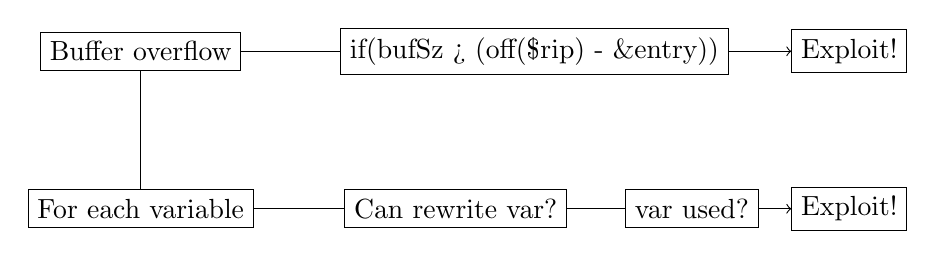
\begin{tikzpicture}
\node at (0,0) [rectangle,draw] (s) {Buffer overflow};
\node at (5,0) [rectangle,draw] (a1) {if(bufSz > (off(\$rip) - \&entry))};
\node at (9,0) [rectangle,draw] (a2) {Exploit!};
\node at (0,-2) [rectangle,draw] (b1) {For each variable};
\node at (4,-2) [rectangle,draw] (b2) {Can rewrite var?};
\node at (7,-2) [rectangle,draw] (b3) {var used?};
\node at (9,-2) [rectangle,draw] (b4) {Exploit!};
\draw[->] (s) -- (a1) -- (a2);
\draw[->] (s) -- (b1) -- (b2) -- (b3) -- (b4);
\end{tikzpicture}

\end{frame}
\begin{frame}{Thank you Questions ?}

See the title

\end{frame}



\end{document}
